\documentclass[aspectratio=169,t,11pt,table]{beamer}
\usepackage{../../slides,../../math}
\definecolor{accent}{HTML}{2B5269}
\definecolor{accent2}{HTML}{9D2235}

\title{Topic 4: Regression Discontinuity}
\subtitle{\it  ECON 5783 — University of Arkansas}
\date{Fall 2024}
\author{Prof. Kyle Butts}

\begin{document}

% -----------------------------------------------------------------------------
\begin{frame}[noframenumbering,plain]
\maketitle

% \bottomleft{\footnotesize $^*$A bit of extra info here. Add an asterich to title or author}
\end{frame}
% -----------------------------------------------------------------------------

\begin{frame}{Regression Discontinuity Design (RDD)}{Example 1}
  Lee (2008, JOE) sutdies the ``incumbency advantage'', the hypothesis that being a serving elected official improves future election outcomes

  \pause
  \bigskip
  The problem, of course, is that candidates who won their election usually are different than those that do not 
  \begin{itemize}
    \item e.g. are more charming, in a more one-sided district, have a better resume
  \end{itemize}

  \pause
  \bigskip
  Lee's idea is to compare candidates who narrowly lost to those that narrowly won 
  \begin{itemize}
    \item By having similar vote percentage, Lee hopes, to be comparing candidates with similar unobservables
  \end{itemize}
\end{frame}

\imageframe{figures/lee_win_tp1.pdf}

\begin{frame}{Regression Discontinuity Design (RDD)}{Example 1}
  There is a clear jump from candidates that narrowly lost to candidates that narrowly won
  \begin{itemize}
    \item The main concern is that candidates that just lost look different in terms of unobservables to those that just won
  \end{itemize}

  \pause
  \bigskip
  To try and alleviate this concern, Lee checks if other observed variables `jump' at the cutoff 
  \begin{itemize}
    \item A jump in other `pre-determined' variables at the cutoff would be problematic to our story
  \end{itemize}
\end{frame}

\imageframe{figures/lee_win_prior_office_exp.pdf}

\begin{frame}{Regression Discontinuity Design (RDD) Terminology}{}
  In the RDD literature, we will have a \alert{`running' variable} (`score' variable), $X_i$, and a \alert{`cutoff'} value $c$
  \begin{itemize}
    \item Units with $X_i < c$ do not receive the `policy` and units with $X_i 
    \geq c$ do
  \end{itemize}

  \bigskip 
  The treatment variable is defined as $D_i = \one{X_i \geq c}$
\end{frame}

\begin{frame}{Regression Discontinuity Design (RDD)}{Example 2}
  Bleemer and Mehta (2022, AEJ Applied) study the returns to being an economics major by leveraging a requirement of a 2.8 GPA threshhold in Econ 1 and 2 at UCSC:

  \begin{itemize}
    \item Comparing students just above a 2.8 GPA to those just below helps address selection into economics major
    
    \item A potential concern is that highly-motivated students near the threshold might ask for higher grade, extra credit, etc.
  \end{itemize}
\end{frame}

\begin{frame}{}
  \begin{columns}[T]
    \begin{column}{.5\textwidth}\vspace*{-\bigskipamount}
      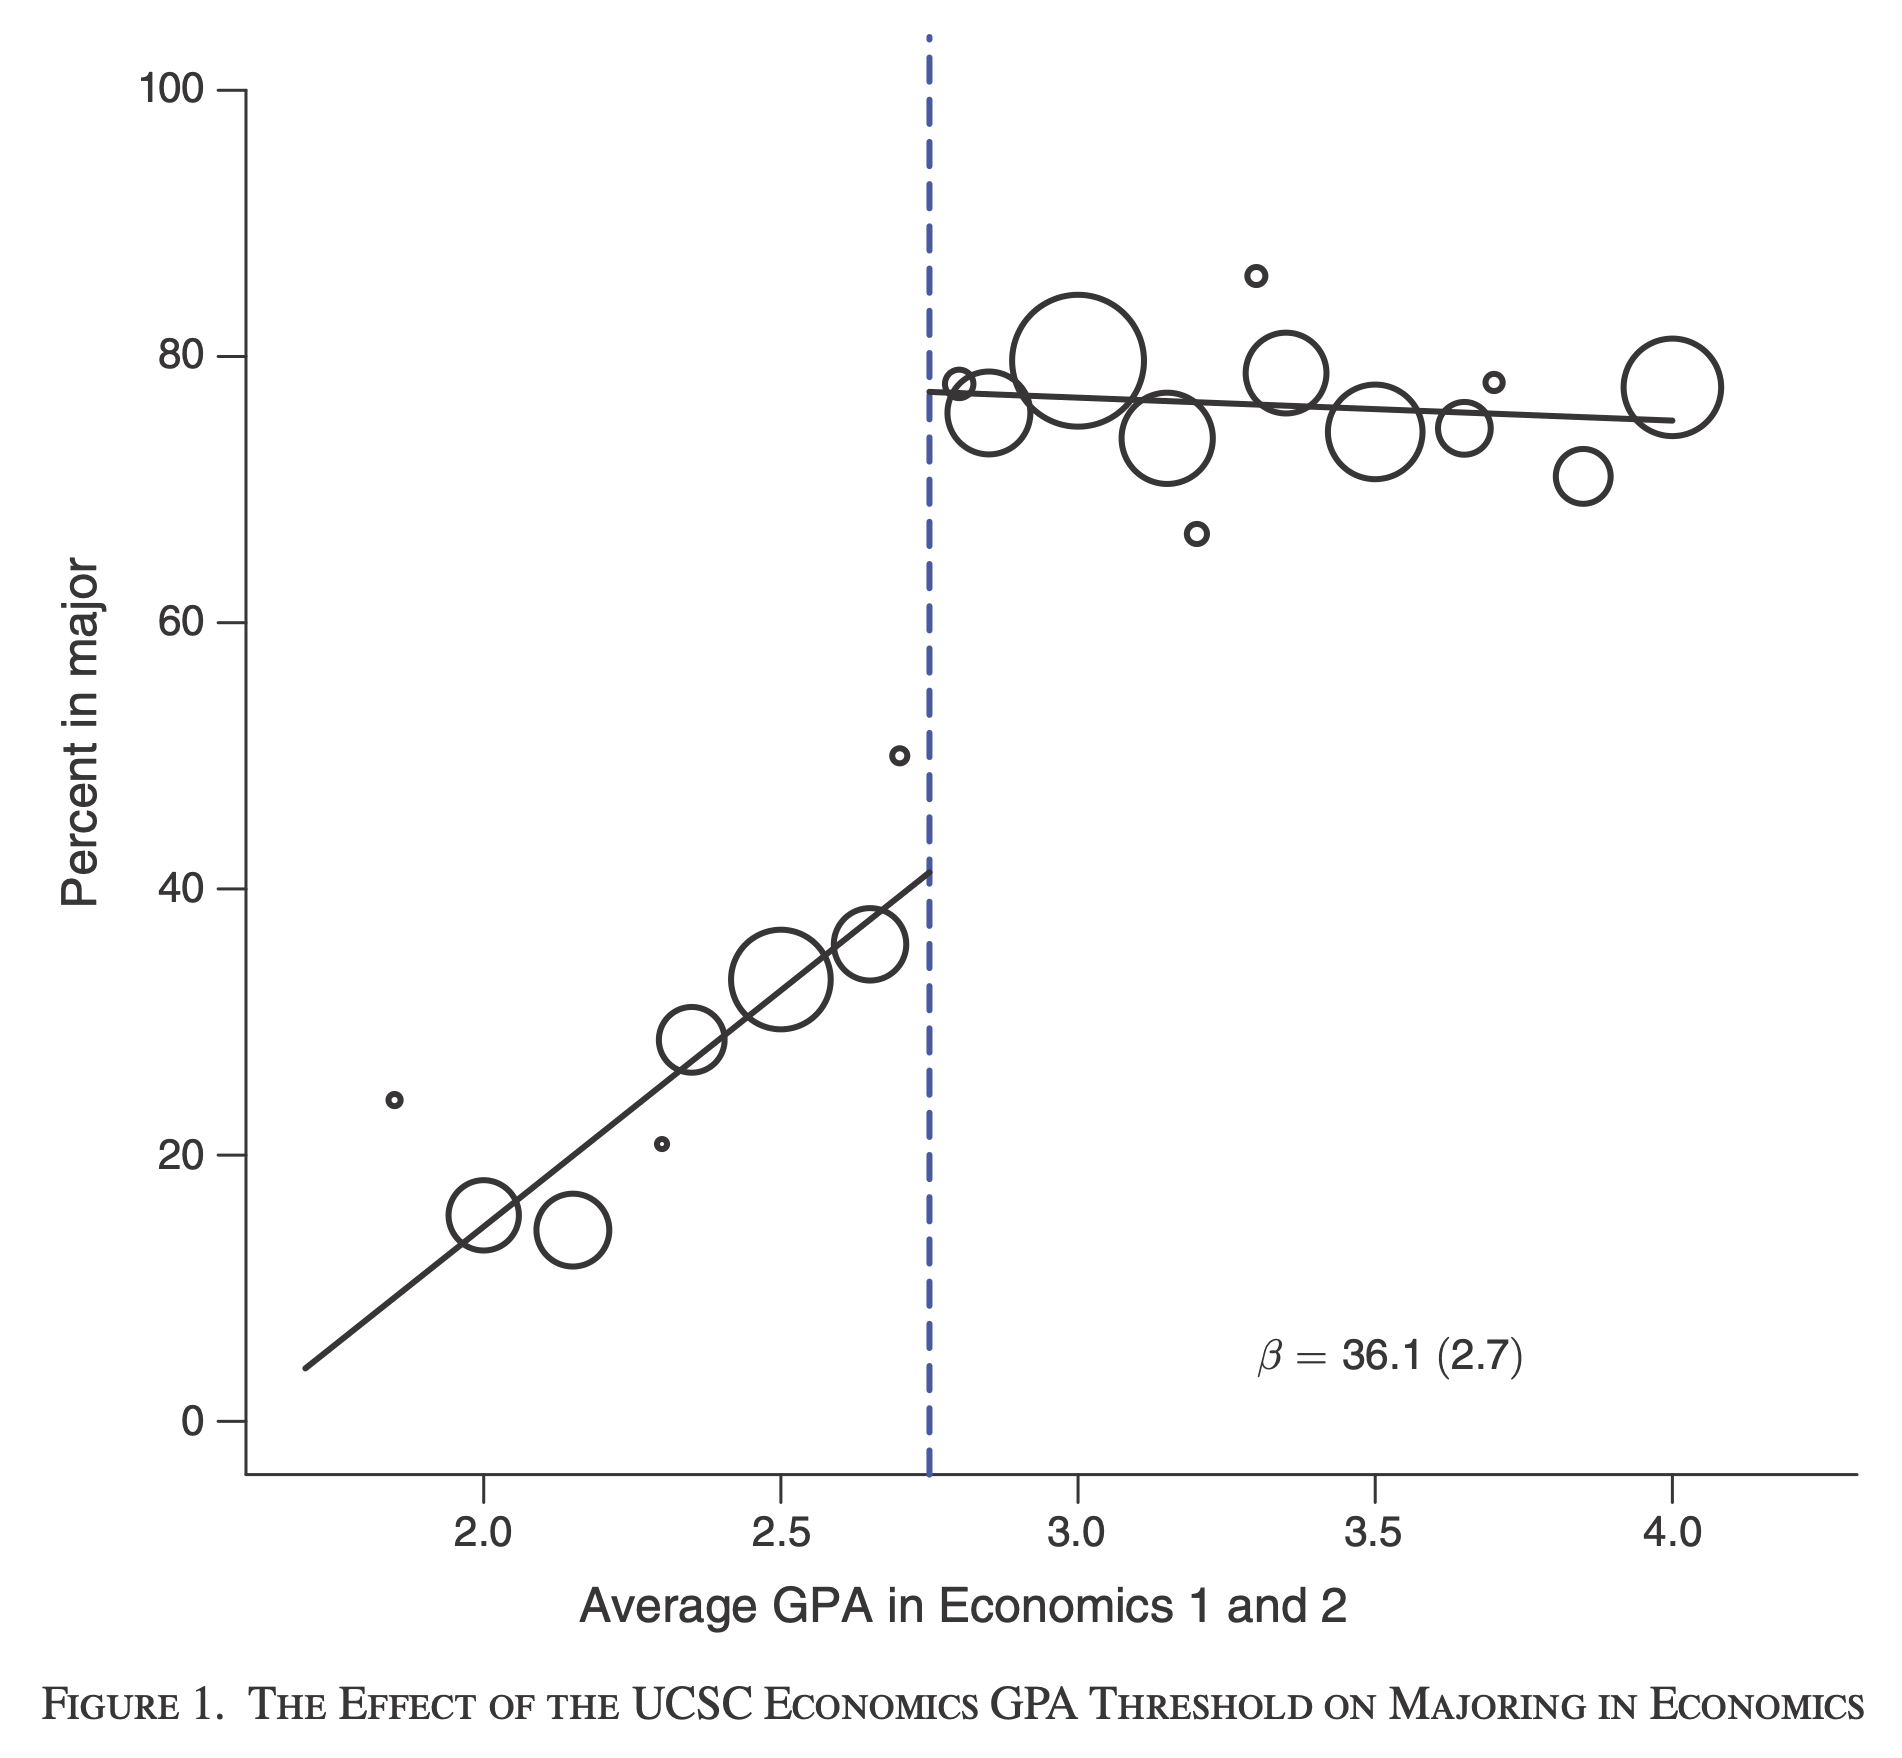
\includegraphics[width = \textwidth]{figures/bleemer_mehta_1.png}
    \end{column}
    \begin{column}{.5\textwidth}\vspace*{-\bigskipamount}
      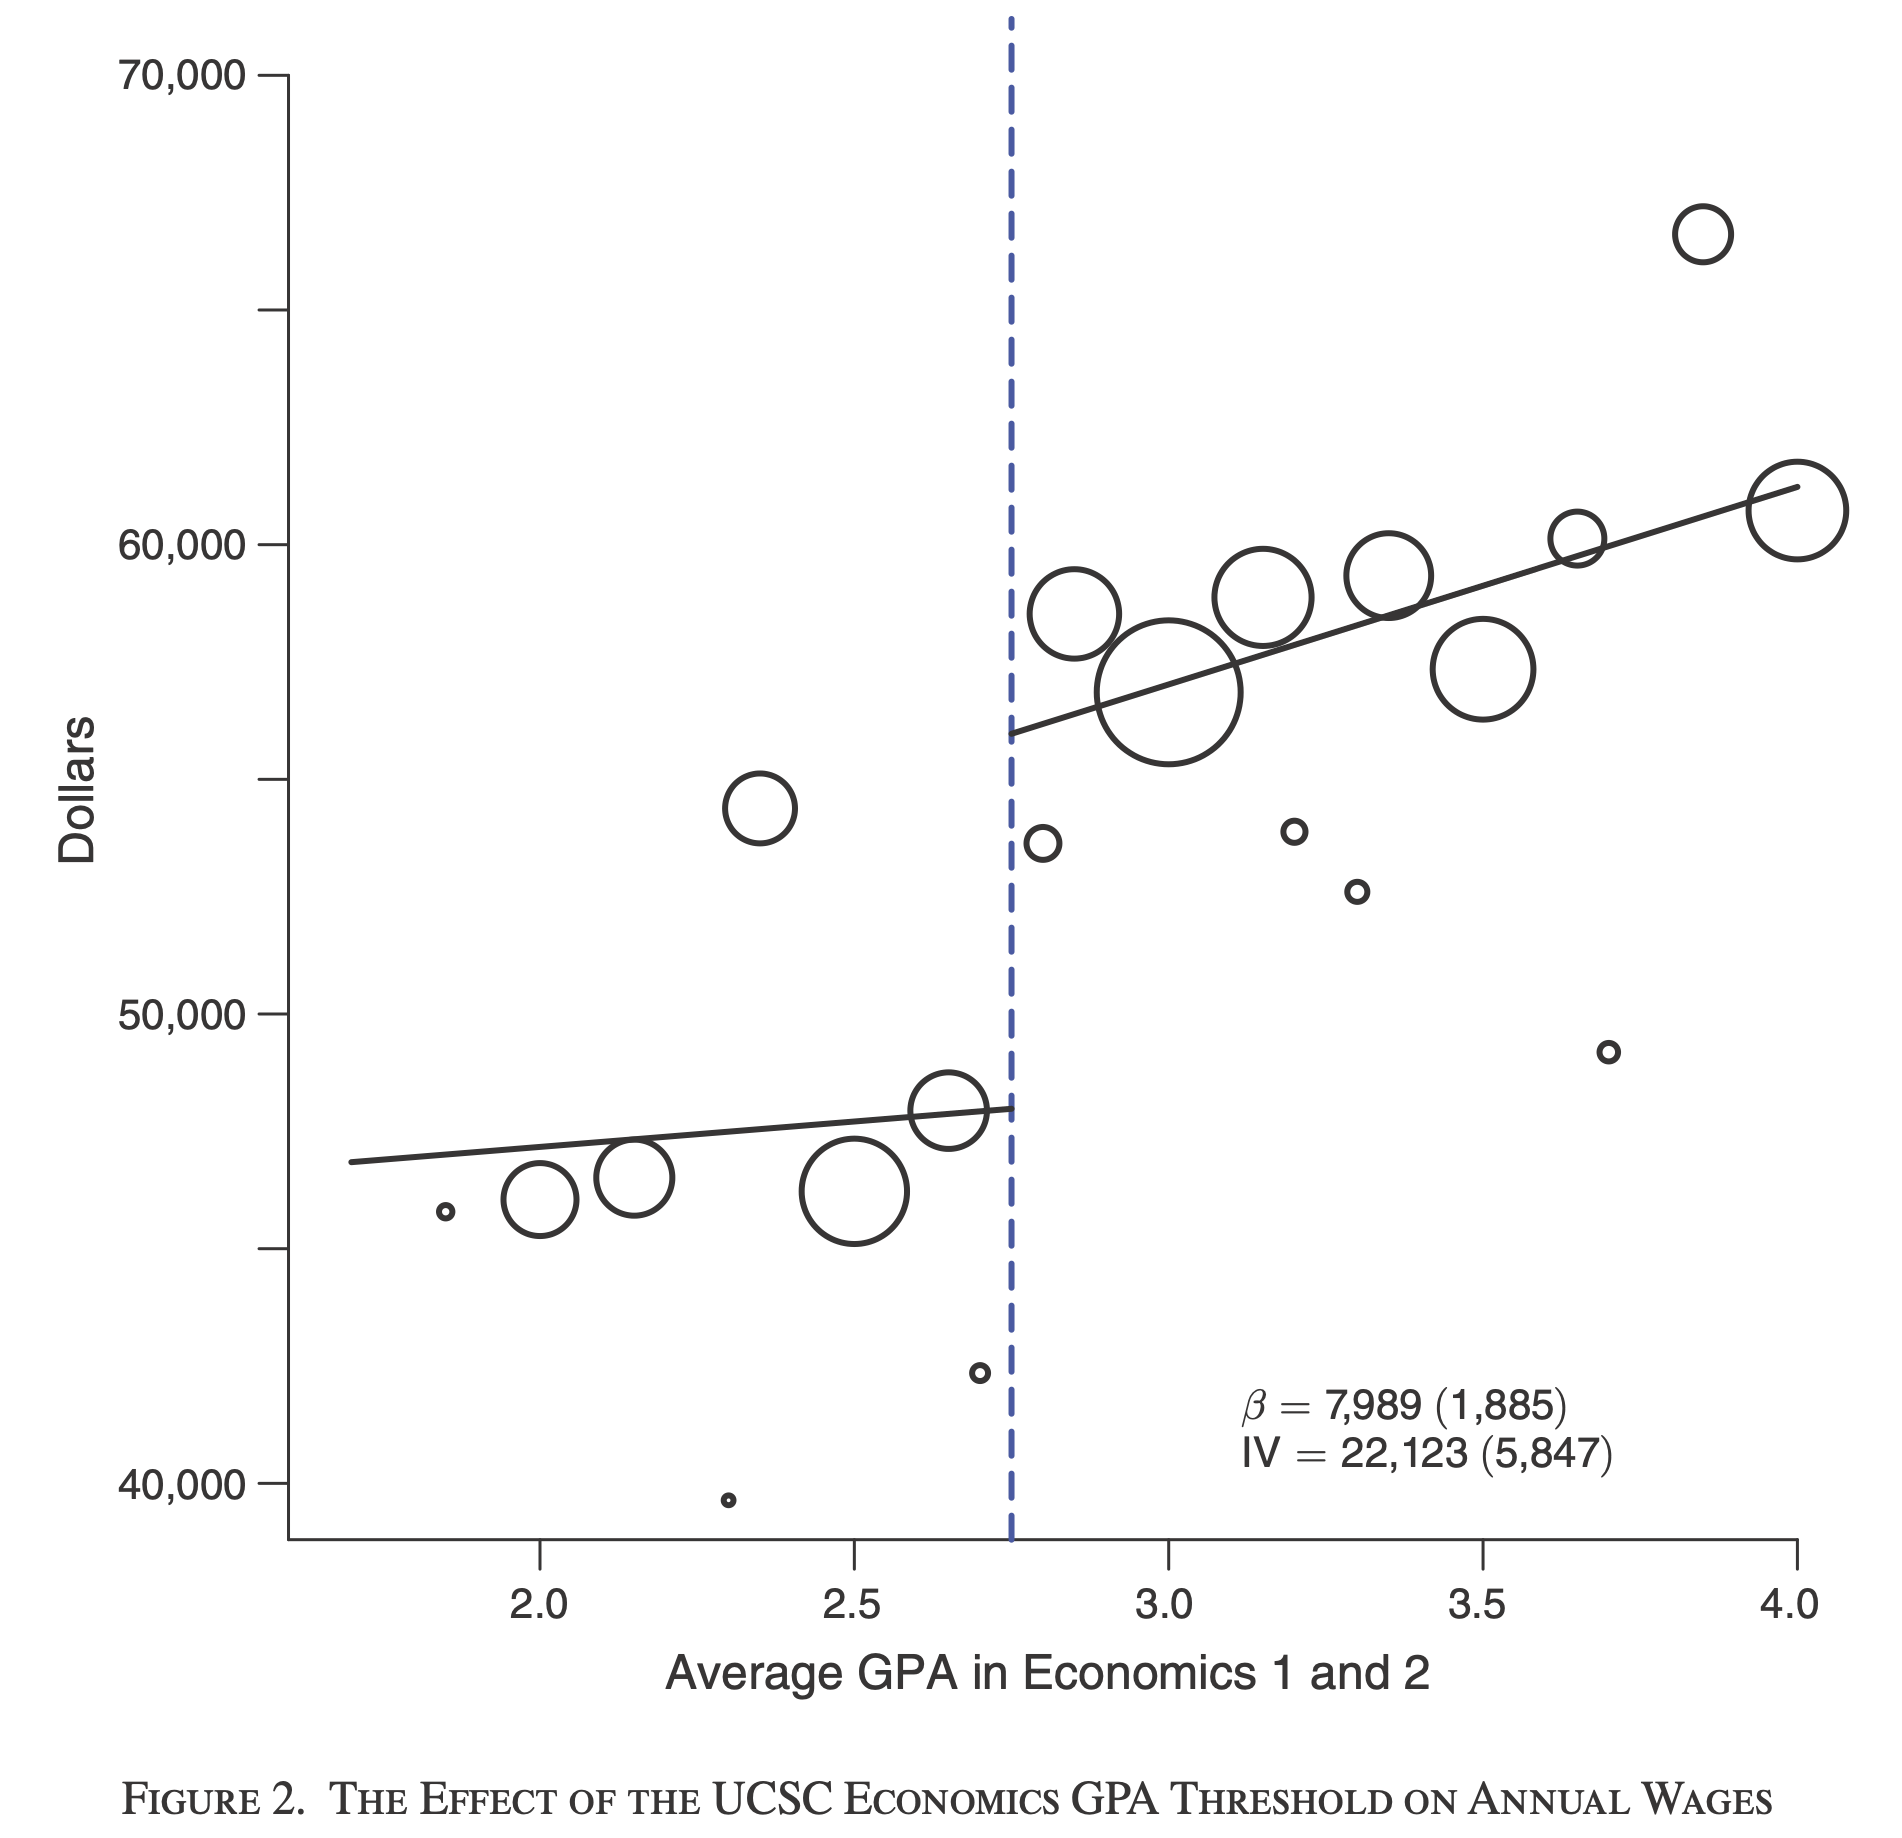
\includegraphics[width = \textwidth]{figures/bleemer_mehta_2.png}
    \end{column}
  \end{columns}
\end{frame}

\begin{frame}{Regression Discontinuity Design (RDD)}{Example 3}
  Hoekstra (2009, RESTAT) estimates the impact of attending a `flagship university' on future earnings
  \begin{itemize}
    \item There was an internal (secret) SAT cutoff that had a large increase in the probability of acceptance
  \end{itemize}

  \bigskip
  That this cutoff was secret helps with concerns over retaking SAT, e.g.  
\end{frame}

\imageframe{figures/hoekstra_2009_1.png}
\imageframe{figures/hoekstra_2009_2.png}

\begin{frame}{Regression Discontinuity Design (RDD)}{Example 4}
  Angrist and Lavy (1999, QJE) study the effect of class size on kid's learning.
  They use a rule in Israel that requires all classes to have 40 or fewer students
  \begin{itemize}
    \item This creates sharp drops in class size at 41, 81, 121, 161 students
  \end{itemize}
\end{frame}

\imageframe{figures/angrist_lavy_1999.png}


\begin{frame}{Regression Discontinuity Design (RDD)}{Example 5}
  Anderson and Magruder (2011, Economics Journal) study the impact of restaurant Yelp ratings on restaurant business outcomes
  \begin{itemize}
    \item Yelp takes the average rating (e.g. 3.27) and shows the nearest number of stars rounding/up or down. E.g. 3.24 rounds down to 3 and 3.25 rounds up to 3.5
  \end{itemize}

  \pause
  \bigskip
  Their argument is that the score, average rating. is a noisy measure of the true quality and so restaurants look the same on either side of the cutoff
  \begin{itemize}
    \item Their main concern is `manipulation' of running variable (we'll come back to this)
  \end{itemize}
\end{frame}

\begin{frame}{Regression Discontinuity Design (RDD)}{Example 6}
  Turner et. al. (2014, ECTA) study the impacts of land-use regulations on the value of land
  \begin{itemize}
    \item They compare homes on one side of a zoning border to homes on the others
    \item The assumption is that the neighborhood doesn't `abruptly' change when crossing the zoning boundary
  \end{itemize}

  \bigskip 
  This is an example of a spatial RDD which we'll discuss more about later
\end{frame}

\begin{frame}{Difficulties with RDD}
  We can not do our usual strategy of comparing treated and untreated individuals with the same $X_i$
  \begin{itemize}
    \item Either everyone is treated or no one is
  \end{itemize}

  \bigskip
  But, there is one point where we \emph{kind of} have treated and untreated units: the cutoff $c$
  \begin{itemize}
    \item This is our intuition for using `just above' versus `just below' the cutoff.
  \end{itemize}
\end{frame}

\section{Formalizing RDD Identification Arguments}

\begin{frame}{Formalizing RDD (Take 1)}{``Noisy'' running variable}
  Let's use a canonical example of students taking a test ($X_i$) and students above a certain cutoff, $c$, are treated (e.g. put in honor's class).

  \bigskip
  Students will vary in terms of their expected score, $\sigma_i = \expec{X_i}$. We think that future outcomes $Y_i$ vary systematically based on $\sigma_i$
  \begin{itemize}
    \item Comparing students above and below the cutoff will be biased  
  \end{itemize}
\end{frame}

\begin{frame}{``Noisy'' running variable creates an experiment}{}
  For random reasons (a weird question, skipped breakfast, etc.) students score is given by $X_i = \sigma_i + \varepsilon_i$, where $\varepsilon$ is random noise.
  \begin{itemize}
    \item For students with $\sigma_i$ close to $c$, $\varepsilon_i$ will make them above or below the cutoff
  \end{itemize}

  \pause
  \bigskip
  This means for $\sigma_i$ close to $c$, we have a \emph{natural experiment}
  \begin{itemize}
    \item Of course, we don't observe $\sigma_i$, so instead we take students within some range $c \pm h$. 
    
    \item If $h$ is ``small enough'', we can do a difference in means between students below and above the cutoff
  \end{itemize}
\end{frame}

\imageframe{figures/plot_dgp_1_rand_tau.pdf}

\begin{frame}{``Local'' treatment effect}{}
  In essence, we throw out all the data outside of $\left[ c-h, c+h \right]$ and compare students with $\sigma_i \approx c$
  
  \bigskip
  This means we only learn about what the impact of treatment is for students with $\sigma_i \approx c$
  \begin{itemize}
    \item E.g. if the cutoff is an SAT score of 1950, then we estimate the impact of treatment for students with around that score
  \end{itemize}
\end{frame}

\begin{frame}{``Local'' treatment effect}{}
  That is, we compare the following:
  \begin{align*}
    &\expec{Y_i}{c < \sigma_i < c+h} - \expec{Y_i}{c-h < \sigma_i < c} \\
    &\quad = \expec{Y_i(1)}{c < \sigma_i < c+h} - \expec{Y_i(0)}{c-h < \sigma_i < c} \\
    \pause
    &\quad \approx \expec{Y_i(1)}{\sigma_i = c} - \expec{Y_i(0)}{\sigma_i = c}
  \end{align*}

  That is, we estimate the CATE for people with $\sigma_i \approx c$
\end{frame}

\begin{frame}{How much `noise' is there in the running variable?}{}
  How do we know how large to make the cut-off $h$? 
  \begin{itemize}
    \item The gold-star answer is to have some application-specific understanding to know how much noise there is and take $h$ to be half that noise
  \end{itemize}

  \bigskip
  Otherwise, we are left to trying to determine a `reasonable' $h$
\end{frame}

\begin{frame}{How much `noise' is there in the running variable?}{}
  There is a trade-off between using a smaller or larger $h$
  \begin{itemize}
    \item On the one hand, a smaller $h$ makes it more likely that units in $(c-h, c)$ look similar to units in $(c, c+h)$
    
    \item On the other, a larger $h$ uses more observations for estimation. A larger $h$ runs a risk of including units that differ systematically from the $\sigma_i = c$ units
  \end{itemize}

  When data on attributes of units are available, then we can use those to help with determining $h$
\end{frame}

\begin{frame}{Estimation of $h$ using extra covariates}{}
  Cattaneo, Frandsen and Titiunik (2015, Journal of Causal Inference) recommend a procedure (available in \texttt{rdlocrand}) where:
  \begin{itemize}
    \item Start with a very small $h_1$ and test if the mean of $\bm{X}_i$ are the same in $(c - h_1, c)$ and $(c, c + h_1)$
    
    \item If you fail to reject the null of no difference in means, then expand to $h_2$
    
    \item Continue until you reject the null
  \end{itemize}

  \bigskip
  The idea being, select the largest $h$ where units `look the same' on both sides of the cutoff.
\end{frame}


\begin{frame}[fragile]{\texttt{rdlocrand} basic syntax}
  \vspace*{-\medskipamount}
  \begin{codeblock}
library(rdlocrand)

# Estimate effect and get p-values
rdrandinf(
  Y = df$y, R = df$score, cutoff = 0, wl = 0.025, wr = 0.025
)

# Estimate optimal h
rdwinselect(
  R = df$score, X = cbind(df$x1, df$x2, df$x3), obsmin = 10, wobs = 5
)
  \end{codeblock}  
\end{frame} 

\begin{frame}{Local randomization argument}
  This approach has a nice intuition: local to the cutoff we have a quasi-experiment due to noise in the running variable

  \bigskip
  Despite this, this approach is less popular than the next approach we discuss
  \begin{itemize}
    \item In part, sometimes we don't believe there is noise in the running variable
    
    \item The plots, like in Lee (2008), are the bread and butter of the RDD
    \begin{itemize}
      \item These are not "difference-in-means" but instead rely on trying to identify a "jump" in smoothed lines
    \end{itemize} 
  \end{itemize}
\end{frame}

\begin{frame}{Formalizing RDD (Take 2)}{Continuity of outcomes}
  The second approach we will discuss is the older (and more commonly used) approach to RDD estimation
  \begin{itemize}
    \item Instead of assumping the score is randomly assigned, this method will rely on a `continuity assumption' of potential outcomes
  \end{itemize}

  \pause
  \bigskip
  The \alert{continuity assumption} says that both the treated and untreated potential outcomes evolve `smoothly' and do not have an abrupt `jump' (discontinuity) at the cutoff
  \begin{itemize}
    \item This is what our mind `tells us to do' when we see these RDD plots
  \end{itemize}
\end{frame}

\imageframe{figures/lee_win_tp1.pdf}

\begin{frame}{Formalizing continuity}
  The goal of our treatment effect estimator is to identify the following:
  $$
    \expec{Y_i(0)}{X_i = c} \ \text{ and }\ \expec{Y_i(1)}{X_i = c}
  $$

  We don't typically observe anyone with $X_i$ exactly equal to 0 (assuming continuous $X_i$)
  \begin{itemize}
    \item So, necessarily we need to extrapolate to the cutoff using observations away from the cutoff
  \end{itemize}
\end{frame}

\begin{frame}{Formalizing continuity}
  Simliar to the selection on observables, define:
  $$
    \mu_d(x) = \expec{Y_i(d)}{X_i = x}
  $$
  to be the conditional expectation of $Y_i(0)/Y_i(1)$ conditional on the running variable being equal to $x$

  \bigskip
  We will fit $\mu_0(x)$ using obseravtions with $X_i < c$ and $\mu_1(x)$ using $X_i > c$
  \begin{itemize}
    \item E.g. fit a linear model of $X_i$ with observations in $(c - h, c)$ / $(c, c+h)$
  \end{itemize}
\end{frame}

\begin{frame}{Extrapolation as limits}
  We are able to learn about the relationship between $Y_i$ and $X_i$ away from the cutoff. We are going to need to take out model and \alert{extrapolate} it to the cutoff 
  \begin{itemize}
    \item Imagine taking averages of $Y_i$ from $(c, c+h)$ to estimate $\expec{Y_i(1)}{X_i = c}$. Assuming infinite data, as $h \to 0$ our average should get closer to closer to the true CEF.
  \end{itemize}
  
  \bigskip
  More formally, under `continuity' we have
  \begin{align*}
    \expec{Y_i(1)}{X_i = c} 
    &= \lim_{s \downarrow c} \expec{Y_i(1)}{X_i = x}
  \end{align*}
  \begin{itemize}
    \item Note here, we are taking the limit from above to only use obs. with $Y_i = Y_i(1)$
  \end{itemize}
\end{frame}

\begin{frame}{RDD Estimand}
  The \alert{regression discontinuity} estimand is formed as follows:
  \begin{align*}
    \tau_{\texttt{RD}} &= 
    \expec{Y_i(1) - Y_i(0)}{X_i = c} \\
    &= \lim_{s\downarrow c} \expec{Y_i}{X_i = x} - \lim_{s \uparrow c} \expec{Y_i}{X_i = x} 
  \end{align*}

  \begin{itemize}
    \item In words, take the difference between the right-hand limit of $\mu_1(x)$ and the left-hand limit of $\mu_0(x)$
  \end{itemize}
\end{frame}

\begin{frame}{Why `continuity'?}
  Since we are fitting a model using observations away from the cutoff $c$, we are \alert{extrapolating} the estimated $\mu_0(x)$ from the range of $X_i$ we used for estimation to the cutoff $X_i = c$
  \begin{itemize}
    \item For this to work, we need the $\mu_d(x)$ to be continuous in a neighborhood around $c$
  \end{itemize}
\end{frame}

% TODO: Generate fake data where SAT cutoff is known and family-income is correlated with retaking the exam near the cutoff
% RD plot of future earnings on going to top college
% RD plot of average family income


\begin{frame}{Why might continuity fail?}{}
  One of the main concerns people have with an RDD empirical application is that units are `sorting' near the cutoff:
  \begin{itemize}
    \item E.g. if there is an SAT cutoff for a scholarship, some kinds of students who were close to making the threshold might retake the SAT multiple times
  \end{itemize}

  \bigskip
  If students who retook look different than those that don't, $\implies$ at a jump in $Y_{i}(0)$ at the cutoff
  \begin{itemize}
    \item $c + \varepsilon$ is `contaminated' by the retakers 
  \end{itemize}
\end{frame}

\begin{frame}{Why might continuity fail?}{}
  In general, the main intuition is that we want there to be no `sorting' around the threshold
  \begin{itemize}
    \item If we think units' characteristics (observable and unobservable) are smooth over the cutoff, then it's reasonable to assume the potential outcomes are smooth too
  \end{itemize}

  \pause
  \bigskip
  For the covariates you do observe, can show that these do not jump at the cutoff
  \begin{itemize}
    \item Hopefully, the unobservables do not as well
  \end{itemize}
\end{frame}

\begin{frame}{Using observations `near' the cutoff}{}
  Returning to the notion of continuity, to estimate $\mu_d(x)$ at the cutoff $X_i = c$, we want to use observations very close to the cutoff
  \begin{itemize}
    \item So that we extrapolate as little as possible
  \end{itemize}

  \bigskip
  In finite samples, there might be very few observations near the cutoff
  \begin{itemize}
    \item In these settings, noise in the data can make it hard to learn information about the data-generating process
  \end{itemize}
\end{frame}

\begin{frame}{Estimation of RDD}
  There are \emph{many} different approaches to estimation of the RD coefficient, but there are a few common questions:
  \begin{enumerate}
    \item How large of a window around the cutoff should we use?
    \begin{itemize}
      \item Smaller window relies on less `extrapolation' but is `noisier' (bias-variance trade-off)
    \end{itemize}
    
    \item How should we fit the model of $\expec{Y_i(d)}{X_i = x}$
    \begin{itemize}
      \item Simpler models are more robust to extrapolation, but may get the functional form wrong
    \end{itemize}
  \end{enumerate}
\end{frame}

\imageframe{figures/mhe_ex_linear.pdf}
\imageframe{figures/mhe_ex_nonlinear.pdf}
\imageframe{figures/mhe_ex_mistake.pdf}

\begin{frame}{Difference-in-means estimation}{}
  For now, take the window to be $(c-h, c+h)$; we will return to the choice of $h$ later in the slides

  \bigskip
  The simplest estimator is the \emph{locally constant estimator}
  $$
    \mu_0(x) = \expechat{Y_i}{X_i \in (c-h, c)} \ \text{ and }\ \mu_1(x) = \expechat{Y_i}{X_i \in (c-h, c)}
  $$
  \begin{itemize}
    \item This is our difference-in-means estimator
  \end{itemize}
\end{frame}

\begin{frame}{Estimation via Regression}{}
  This can be estimated with the simple regression:
  $$
    Y_i = \alpha_0 + \alpha_1 D_i + u_i
  $$
  on the subsample with $X_i \in (c-h, c+h)$
\end{frame}

\imageframe{figures/plot_dgp_2_tau.pdf}
\imageframe{figures/plot_dgp_2_local_constant_estimator.pdf}

\begin{frame}{Locally-linear estimation}{}
  Now, let's use a linear-model $\mu_d(x) = \alpha_d + \beta_d X_i$
  \begin{itemize}
    \item Note we let the slope vary for $Y_i(0)$ and $Y_i(1)$
  \end{itemize}

  \bigskip
  Take our estimated models and form the regression adjustment estimator as:
  \begin{align*}
    \hat{\tau} 
    &= \left( \hat{\alpha}_1 + \hat{\beta}_1 c \right) - \left( \hat{\alpha}_0 + \hat{\beta}_0 c \right)
  \end{align*}
  \begin{itemize}
    \item This looks like our regression adjustment estimator!
  \end{itemize}
\end{frame}

\begin{frame}{Estimation via Regression}{}
  The locally linear estimator can be estimated with an interacted regression (like with regression adjustment):
  $$
    Y_i = \alpha_0 + \alpha_1 D_i + \beta_0 (X_i - c) + \beta_1 D_i (X_i - c) + u_i
  $$
  on the subsample with $X_i \in (c-h, c+h)$

  \begin{itemize}
    \item Note we recenter, $X_i - c$, so that $\hat{alpha}_1$ is the RDD estimate (e.g. "margin of victory" instead of "vote-share" in Lee, 2008)
  \end{itemize}
\end{frame}

\imageframe{figures/plot_dgp_2_local_linear_estimator.pdf}

\begin{frame}{Why linear if our data looks wiggly?}
  There is a lingering question, if we think our data is very `wiggly' why are we assuming linearity in $X_i$?

  \begin{itemize}
    \item Remember we are using only observations \emph{local} to the cutoff, so (at least asymptotically) wiggly functions are approximately linear on small bandwidths
    
    \item Essentially we are using the logic of the Taylor expansion that we can approximate a function locally using a lienar function
  \end{itemize}
\end{frame}


\begin{frame}{Different Bandwidths}{}
  Our estimator, implicitly depends on our choice of bandwidth $h$
  \begin{itemize}
    \item Larger $h$ uses more observations so should help with precision of our estimate
    \item but relies more on functional form for extrapolation (Taylor approximation only holds locally)
  \end{itemize}
\end{frame}

\imageframe{figures/plot_dgp_2_local_constant_large_bw.pdf}
\imageframe{figures/plot_dgp_2_local_linear_large_bw.pdf}

\begin{frame}{Local polynomial estimation}{}
  We can extend our logic to higher-order polynomials:
  $$
    Y_i = \alpha_0 + \alpha_1 D_i \sum_{p = 1}^\rho \beta_{0,p} (X_i - c)^p + \sum_{p = 1}^\rho \beta_{1,p} (X_i - c)^p + u_i
  $$
  
  Still, $\hat{\alpha_1}$ is our RDD estimator
\end{frame}

\imageframe{figures/plot_dgp_2_local_quadratic_estimator.pdf}

\begin{frame}{RDD By Hand}{}
  The most `straight forward' way to estimate the RDD is to do two regressions:
  \begin{enumerate}
    \item Regress $Y_i$ on a $k$-th order polynomial of $X_i - c$ for $c - h < X_i < c$
    \item Regress $Y_i$ on a $k$-th order polynomial of $X_i - c$ for $c < X_i < c + h$
  \end{enumerate}

  \bigskip
  Predict $Y$ at $X_i = 0$ for both models. These are your estimates for $\hat{\mu}^-$ and $\hat{\mu}^+$ respectively. Then our RD estimate can be formed as
  $$
    \hat{\tau}_{\texttt{RD}} = \hat{\mu}^+ - \hat{\mu}^-
  $$
\end{frame}


\begin{frame}{Example: Punishment and Deterrence: Evidence from Drunk Driving}
  Hansen (2015, AER) considers the impact of getting a DUI (driving while drunk) has on future drinking behavior
  \begin{itemize}
    \item Uses the `legal limit' of a blood-alcohol content of 0.08 as the RDD `cutoff'
  \end{itemize}
\end{frame}

\imageframe{figures/hansen_raw_avgs.pdf}

\begin{frame}[fragile]{RDD by hand: Randomization-based estimation}
	\begin{codeblock}
feols(
  recidivism ~ 1 + over_limit,
  data = subset(hansen, bac1 >= 0.07 & bac1 <= 0.09)
)
	\end{codeblock}
\end{frame}

\begin{frame}[fragile]{RDD by hand: Randomization-based estimation}
  \begin{codeblock}[{}]
OLS estimation, Dep. Var.: recidivism
Observations: 18,897
Standard-errors: IID 
                Estimate Std. Error  t value   Pr(>|t|)    
(Intercept)     0.114784   0.003253 35.28149  < 2.2e-16 ***
over_limitTRUE -0.017903   0.004472 -4.00349 6.2652e-05 ***
---
Signif. codes:  0 '***' 0.001 '**' 0.01 '*' 0.05 '.' 0.1 ' ' 1
  \end{codeblock}
\end{frame}

\begin{frame}[fragile]{RDD by hand: Locally-linear estimation}
  \vspace{-\bigskipamount}
	\begin{codeblock}
feols(
  recidivism ~ 1 + over_limit + 
    I(bac1 - 0.08) + I(bac1 - 0.08) * over_limit,
  data = subset(hansen, bac1 >= 0.04 & bac1 <= 0.12)
)
	\end{codeblock}
\end{frame}

\begin{frame}[fragile]{RDD by hand: Locally-linear estimation}
  \begin{codeblock}[{}]
OLS estimation, Dep. Var.: recidivism
Observations: 72,880
Standard-errors: IID 
                                Estimate Std. Error  t value   Pr(>|t|)    
(Intercept)                    0.113956   0.003718 30.65215  < 2.2e-16 ***
over_limitTRUE                -0.020381   0.004694 -4.34212 1.4131e-05 ***
I(bac1 - 0.08)                -0.312061   0.226113 -1.38011 1.6756e-01    
over_limitTRUE:I(bac1 - 0.08)  0.707713   0.254253  2.78350 5.3790e-03 ** 
---
Signif. codes:  0 '***' 0.001 '**' 0.01 '*' 0.05 '.' 0.1 ' ' 1
  \end{codeblock}
\end{frame}

\begin{frame}[fragile]{RDD plot using \texttt{rdplot} from \texttt{rdrobust}}{}
	\begin{codeblock}
library(rdrobust)
rdplot(y = hansen$recidivism, x = hansen$bac1, c = 0.08, h = 0.4)
	\end{codeblock}
\end{frame}

\imageframe{figures/hansen_rdplot_bw_0pt4.pdf}

\begin{frame}[fragile]{RDD using \texttt{rdrobust}}{}
  \begin{codeblock}
est <- rdrobust(
  y = hansen$recidivism, x = hansen$bac1, c = 0.08
)
summary(est)
  \end{codeblock}
\end{frame}

\begin{frame}[fragile]{RDD using \texttt{rdrobust}}{}
  \begin{codeblock}[{}]
... Details ...

=============================================================================
        Method     Coef. Std. Err.         z     P>|z|      [ 95% C.I. ]       
=============================================================================
  Conventional    -0.018     0.006    -3.083     0.002    [-0.030 , -0.007]    
        Robust         -         -    -2.452     0.014    [-0.031 , -0.003]    
=============================================================================
  \end{codeblock}
\end{frame}


\begin{frame}{Sorting based on the running variable}{}
  As we discussed before, our main threat to the continuity assumption is that units are `sorting' onto either side of the cutoff based on their observable characteristics

  There are two standard `gut checks' that folks will want to see
\end{frame}

\begin{frame}{Check 1: Balance}{}
  First, if we have any `pre-determined' covariates, we want see that there are no jumps in the average of covariates at the cutoff
  \begin{itemize}
    \item Rerun RDD estimator using $X_i$ as the outcome variable. Test $\hat{\tau}_{\texttt{RD}}= 0$
  \end{itemize}

  \bigskip
  Use covariates that you would likely see a jump in if there was sorting (e.g. a proxy for `motivation' for SAT example)
\end{frame}

\imageframe{figures/hansen_balance_check_male.pdf}
\imageframe{figures/hansen_balance_check_white.pdf}

\begin{frame}{Check 2: McCrary Density}{}
  If you don't have extra covariates, you can check for `continuous density' a la McCrary (2006, JOE)

  \bigskip
  The idea is that if we think there is no sorting, then we would expect to see no strong `jump' in the histogram of the running variable
  \begin{itemize}
    \item A jump at the discontinuity suggests that agents are sorting onto one side of the border (assuming the density would be smooth in the absence of the cutoff policy)
  \end{itemize}
\end{frame}

\imageframe{figures/hansen_hist_bac1.pdf}
\imageframe{figures/hansen_rddensity_bac1.pdf}

\begin{frame}{Example}{Camacho and Conover (2011, AEJ: EP)}
  Camacho and Conover (2011, AEJ: EP) discuss a real example of `manipulation'
  \begin{itemize}
    \item Towns in Colombia receive social programs if their poverty index score is below a cutoff
     
    \item The poverty index algorithm becomes public in 1997
  \end{itemize}
\end{frame}

\imageframe{figures/camacho_conover_2011.png}

\begin{frame}{Example}{Camacho and Conover (2011, AEJ: EP)}
  The authors show in their paper that the towns that corruptly gamed their score looked different than those that did not
  \begin{itemize}
    \item Those that gamed their scores had more political competition
  \end{itemize}

  \bigskip
  In this setting, if we saw a big jump at the poverty index cutoff, then we can't know if it's from the social programs or from the higher-level of political competition 
\end{frame}

\begin{frame}{Optimal Bandwidth selection}
  As we discussed before, there is a tension with selection of bandwidth:
  \begin{itemize}
    \item Smaller bandwidths use data closer to the cutoff and rely less on functional form
    
    \item Larger bandwidths lets you use more data to estimate RD
  \end{itemize}

  \bigskip
  All identification relies on the bandwidth getting smaller as the sample size grows
  \begin{itemize}
    \item But we are left wondering what the `optimal bandwidth' is given a finite sample
  \end{itemize}
\end{frame}


\begin{frame}{Optimal Bandwidth selection}
  Calonico, Cattaneo and Farrell (2018, Economics Journal) use statistical methods to identify the `optimal' bandwidth. The optimal bandwith is based on the following:
  \begin{itemize}
    \item Of course, the bandwidth should shrink as the sample size grows

    \item If the curvature of $\expec{Y_i}{X_i = x}$ is more wiggly, the bandwidth should be smaller

    \item If the variance of $Y_i$ near the cutoff is larger, then you should use a larger bandwidth
  \end{itemize}

  \pause
  \bigskip 
  The upshot is this is done automatically for you with \texttt{rdrobust}
  \begin{itemize}
    \item See Cattaneo et. al.'s review article for more details
  \end{itemize}
\end{frame}

% TODO: Discuss discrete running variable?


\section{Spatial RDD}

\begin{frame}{Spatial RDD}{Example}
  Dell (2010, ECTA) considers the impact of historical colonizer institutions on long-run impacts:
  \begin{itemize}
    \item In now Peru and Bolivia, there was a set of Spanish mines that had a catchment area called the `Mita'
  \end{itemize}

  \bigskip
  The boundary was drawn somewhat arbitrarily around the mines, so either side of the Mita boundary should have the same `latent opportunity' (in 2000) except for the fact of the Mita boundary 
  \begin{itemize}
    \item This argument is that $\expec{Y(0)}$ would be continuous right around the border 
  \end{itemize}
\end{frame}

\imageframe{figures/dell_2010_1.png}
\imageframe{figures/dell_2010_2.png}

\begin{frame}{Spatial RDD Setup}
  Units have a location in geographic space $(x_{1,i}, x_{2,i})$ and there is some border consisting of lines in $X_1/X_2$ space

  \begin{itemize}
    \item The borders will separate units into $D_i = 0$ and $D_i = 1$ space.
  \end{itemize}

  \pause
  \bigskip
  Since we are in two-dimensions, it's not immediately clear how to think about ``approaching the border''. For now, let's use the Euclidean distance to the closest point on the border
  \begin{itemize}
    \item Positive distances are within $D_i = 1$ area; negative distances are outside $D_i = 1$ areas
  \end{itemize}
\end{frame}

\begin{frame}{Spatial RDD Idea}
  Let $\text{dist}_i$ be the distance to the closest border with a positive sign if on the $D_i = 1$ area and negative sign if in the $D_i = 0$ area
  \begin{itemize}
    \item The cutoff $c$ is therefore $\text{dist}_i = 0$
  \end{itemize}

  \bigskip
  The RDD identification assumption is the same as before viewing $\text{dist}_i$ as the single running variable
  \begin{itemize}
    \item We assume $\expec{Y_i}{\text{dist}_i = d}$ does not jump at the boundary
  \end{itemize}
\end{frame}

\begin{frame}{Discontinuity in Dell (2010)}
  In the context of Dell (2010), the assumption is that in the absence of the Mita boundaries, the outcomes
  \begin{itemize}
    \item Most of the boundary was at the base of the Andes mountain, so this assumption is implausible there
    \item Dell argues that the part of the boundary she uses was a bit `randomly drawn' in the sense that it was not place on some obvious cutoff
  \end{itemize}

  \bigskip
  To bolster her argument, she presents some evidence that the boundary was not 
\end{frame}

\begin{frame}{Discontinuities are much more likely with spatial boundaries}
  Turner et. al. (2014, ECTA) used data at the city/town-level for their analysis, so their borders primarily were at the town level
  \begin{itemize}
    \item They need to make the strong assumption that on either side of a town-border did not differ in ways that would impact home prices in a way that is correlated with zoning laws
  \end{itemize}

  \bigskip
  This seems unlikely because, for example, towns with more restrictive zoning laws tend to have higher school budgets
\end{frame}

\begin{frame}{Multiple Treatments at Boundaries}
  We have already discussed one concern regarding sorting onto sides of the border. Another common problem is that multiple treatments might turn on at a border
  \begin{itemize}
    \item E.g. many policy differences across town borders
  \end{itemize}
\end{frame}

\begin{frame}{Multiple Treatments at Boundaries}
  Grembi et. al. (2018, AJPS) look at a common occurence of `population threshholds' for policies to take place 
  \begin{itemize}
    \item Since policymakers chose arbitrary numbres, they usually pick nice round numbers
    \item Also common is some mulitple of the federal poverty line
  \end{itemize}

  \bigskip
  This creates a bundle of different treatments that turn on at a threshhold
  \begin{itemize}
    \item How do you disentangle effects from different policies?
  \end{itemize}
\end{frame}

\begin{frame}{}
  \begin{columns}[T]
    \begin{column}{0.53\textwidth}
      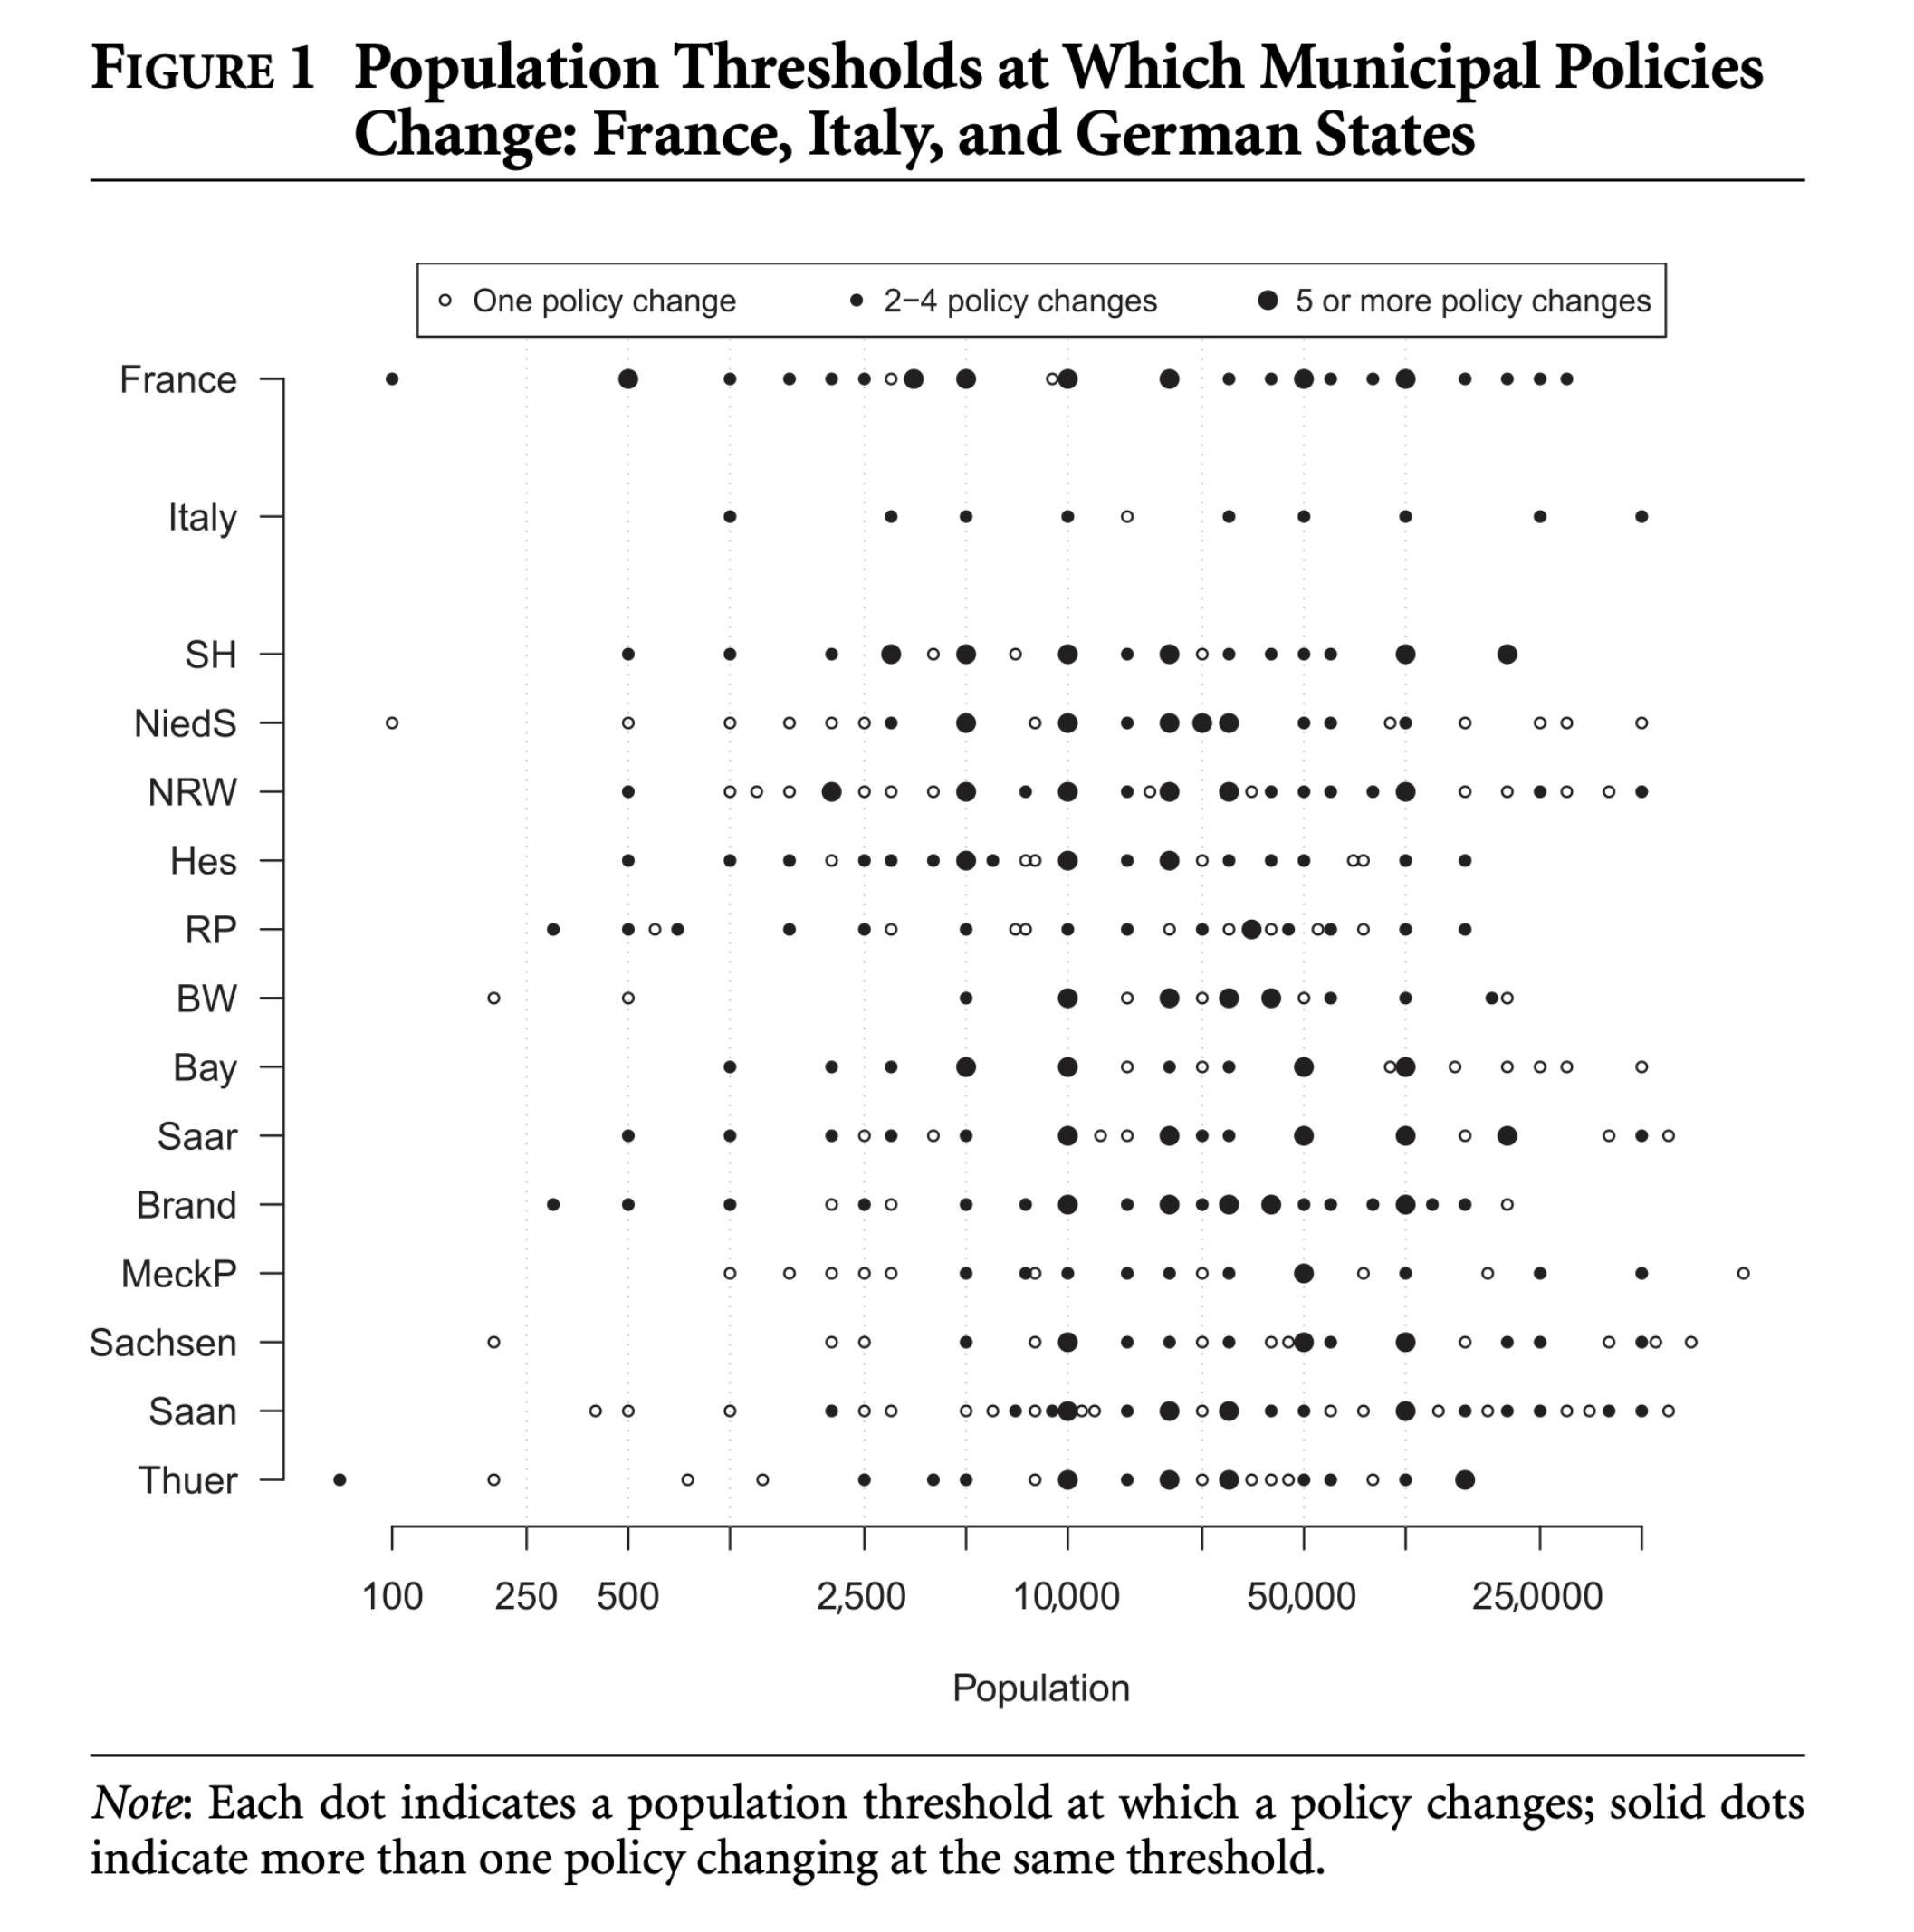
\includegraphics[width = \textwidth]{figures/grembi_et_al_2018.png}
    \end{column}
    \hfill
    \begin{column}{0.45\textwidth}
      \bigskip
      From Grembi et. al. (2018, AJPS)
      
      \bigskip
      Many `round' population threshholds have multiple policy changes
    \end{column}
  \end{columns}
\end{frame}


\begin{frame}{Solution Idea \#1: Find better cutoffs}
  The first idea is to find better borders where we more confidently think there aren't other policy changes

  \bigskip
  E.g. Kulka, Sood, and Chiumenti (2023, WP) look at the impact of zoning changes on home prices like in Turner et. al.
  \begin{itemize}
    \item They have zoning microdata and only compare zoning borders that fall within town and school-districts 
    \begin{itemize}
      \item Compare homes within the same town and school district on opposite side of zoning borders
    \end{itemize}
  \end{itemize}

\end{frame}

\begin{frame}{Solution Idea \#2: Compare before and after a policy is put into place}
  In some cases, you can observe units before vs. after a new policy is put into place

  \bigskip
  If all other policies are in place and all sorting has already taken place, we can estimate an RD before and an RD after
  \begin{itemize}
    \item The RD before the new policy is put into place tells you about the jump in $Y_i(0)$ that already exists (from sorting and the treatment effect of other policies)
    
    \pause
    \item The RD after the new policy still has the previous jump, but also a new jump from the new policy
  \end{itemize}

  \bigskip
  The `difference-in-jumps` estimates the effect of the new policy
\end{frame}

\begin{frame}{Difference in discontinuities}
  This method was first proposed by Grembi et. al. (2016, AEJ Applied) and they coined it `difference in discontinuities' (we will see why later)

  \bigskip
  This relies on two assumptions:
  \begin{enumerate}
    \item The jump in $Y_i(0)$ stays constant over time, so that we can estimate it using the pre-period
    \begin{itemize}
      \item There is no \emph{new} effect and no \emph{new} sorting from \emph{previous} treatments
    \end{itemize}
    
    \item The $Y_i(1)$ curve will also have a jump of the same magnitude as $Y_i(0)$
    \begin{itemize}
      \item There is no \emph{additional} sorting occuring from the \emph{new} policy
    \end{itemize}
  \end{enumerate}
\end{frame}

\begin{frame}{RDD at $t = 0$}
  \begin{columns}[T]
    \begin{column}{.65\textwidth}\vspace*{-\bigskipamount}
      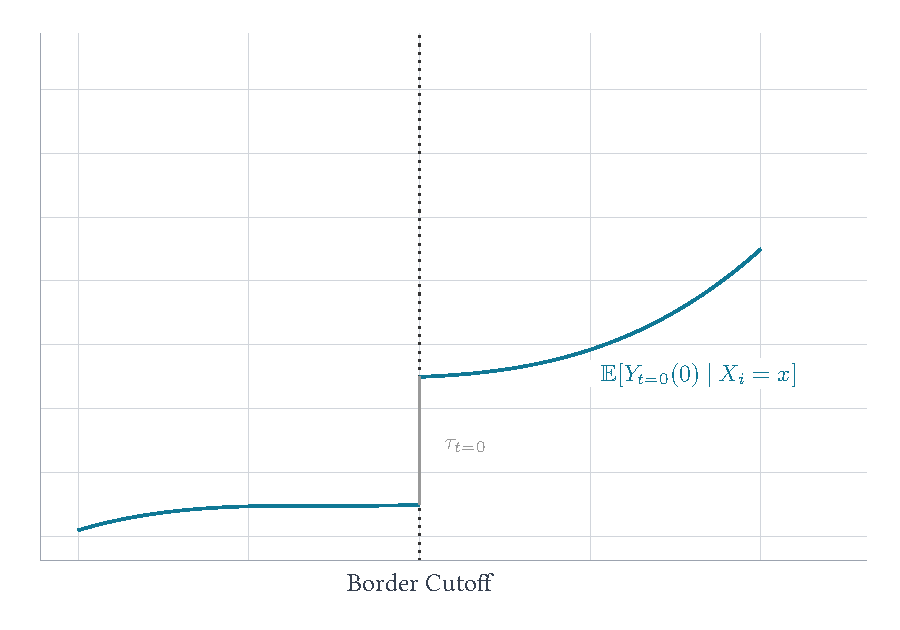
\includegraphics[width = \textwidth]{figures/diff_in_disc_pre.pdf}
    \end{column}
    \begin{column}{.35\textwidth}
      Pre-treatment RD informs us of effects of other policy changes and non-treatment based-sorting
    \end{column}
  \end{columns}
\end{frame}

\begin{frame}{RDD at $t = 1$}
  \begin{columns}[T]
    \begin{column}{.65\textwidth}\vspace*{-\bigskipamount}
      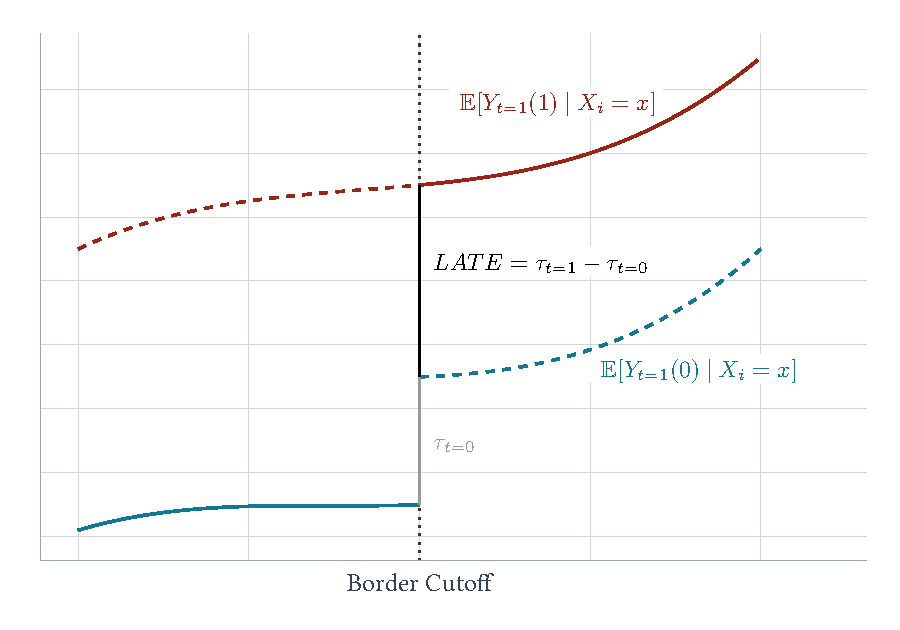
\includegraphics[width = \textwidth]{figures/diff_in_disc_post.pdf}
    \end{column}
    \begin{column}{.35\textwidth}
      Difference of post RD and pre RD is the treatment effect of interest
    \end{column}
  \end{columns}
\end{frame}


\begin{frame}{Implementing Diff-in-disc}
  Butts (2021, AEL) (that's me) shows an easy way to estimate the difference-in-discontinuities:

  \begin{itemize}
    \item Instead of doing two RDs and taking the difference, do an RD on first-differenced data 
  \end{itemize}

  \bigskip
  I.e. use \texttt{rdrobust} using \texttt{df\$y1 - df\$y0} as the outcome variable
\end{frame}

\end{document}
    
